% Copyright 2004 by Till Tantau <tantau@users.sourceforge.net>.
%
% In principle, this file can be redistributed and/or modified under
% the terms of the GNU Public License, version 2.
%
% However, this file is supposed to be a template to be modified
% for your own needs. For this reason, if you use this file as a
% template and not specifically distribute it as part of a another
% package/program, I grant the extra permission to freely copy and
% modify this file as you see fit and even to delete this copyright
% notice. 

\documentclass[xcolor=dvipsnames]{beamer}
\usepackage{bibentry}
\setbeamertemplate{bibliography item}{\insertbiblabel}
\usepackage{cancel}
\usepackage{amsmath} 
\usepackage{mathtools}
\newcommand{\norm}[1]{\left\lVert #1 \right\rVert}
% Command for round parenthesis
\newcommand{\roundP}[1]{\left( #1 \right)}
% Command for poisson brackets
\newcommand{\poisson}[2]{\left\lbrace #1, #2 \right\rbrace}

\usepackage{varwidth}
\usepackage{lipsum}
\usepackage{color}
\usepackage{todonotes}
\definecolor{dgray}{gray}{0.30}
\definecolor{uyellow}{RGB}{253,241,0}

\usepackage[utf8]{inputenc}
\usepackage{graphicx}
\usepackage{epstopdf}
\usepackage[english]{babel}
\usepackage{hyperref}
\usepackage{datenumber}
\usepackage{todonotes}
\usepackage{mathtools}
\usepackage{amsmath}
\usepackage{amssymb}
\usepackage{amsthm}
\usepackage[caption=false]{subfig}

\newtheorem*{thm}{Theorem}
\newcommand{\fmunu}{F^{\mu\nu}}
\newcommand{\E}{\vec{E}}
\newcommand{\B}{\vec{B}}
\newcommand{\rot}{\nabla\times}
\newcommand{\dive}{\nabla\cdot}
\newcommand{\tmunu}{T^{\mu\nu}}
\newcommand{\levichi}{\epsilon_{\mu\nu\sigma\gamma}}
\newcommand{\dete}{\textrm{det}}
\newcommand{\lna}{\textrm{ln}}
\newcommand{\Tr}{\textrm{Tr}}
\newcommand{\seno}{\textrm{sin}}

\makeatletter
\newcommand{\pushright}[1]{\ifmeasuring@#1\else\omit\hfill$\displaystyle#1$\fi\ignorespaces}
\newcommand{\pushleft}[1]{\ifmeasuring@#1\else\omit$\displaystyle#1$\hfill\fi\ignorespaces}
\makeatother



% There are many different themes available for Beamer. A comprehensive list with examples is given here:
% http://deic.uab.es/~iblanes/beamer_gallery/index_by_theme.html
%\usetheme{AnnArbor}
%\usetheme{Antibes}
%\usetheme{Bergen}
%\usetheme{Berkeley}
%\usetheme{Berlin}
%\usetheme{Boadilla}
%\usetheme{boxes}
%\usetheme{CambridgeUS}
\usetheme{Copenhagen}
%\usetheme{Darmstadt}
%\usetheme{default}
%\usetheme{Frankfurt}
%\usetheme{Goettingen}
%\usetheme{Hannover}
%\usetheme{Ilmenau}
%\usetheme{JuanLesPins}
%\usetheme{Luebeck}
%\usetheme{Madrid}
%\usetheme{Malmoe}
%\usetheme{Marburg}
%\usetheme{Montpellier}
%\usetheme{PaloAlto}
%\usetheme{Pittsburgh}
%\usetheme{Rochester}
%\usetheme{Singapore}
%\usetheme{Szeged}
%\usetheme{Warsaw}
%\usecolortheme{seagull}
%\usetheme{Malmoe} 

\setbeamercolor{frametitle}{fg=Black,bg=Blue!60}
\setbeamercolor{section in head/foot}{bg=Blue, fg=Black}
\setbeamercolor{author in head/foot}{bg=blue, fg=Black} 
\setbeamercolor{date in head/foot}{fg=blue} 
\setbeamercolor{institute in head/foot}{fg=Black}
\usecolortheme[named=Black]{structure}
\setbeamerfont{footnote}{size=\footnotesize}

\setbeamertemplate{}[page number] % To replace the footer line in all slides with a simple slide count uncomment this line
 
\title{\textbf{The Expected Shape of the Milky Way's Dark Matter Halos }}

% A subtitle is optional and this may be deleted
%\subtitle{Optional Subtitle}

\author{Jesus Prada}
% - Give the names in the same order as the appear in the paper.
% - Use the \inst{?} command only if the authors have different affiliation.

\institute[{\color{Black} Universidad de los Andes}] % (optional, but mostly needed)
{
 \normalsize Advisors:\\
 PhD Jaime E. Forero-Romero \\ \small Universidad de los Andes, Departamento de Física\\
  \vspace{5mm}
 \normalsize PhD Volker Springel \\ \small  Heidelberg's Institute of Theoretical studies
}
% - Use the \inst command only if there are several affiliations.
% - Keep it simple, no one is interested in your street address.

\tiny
\date{ \footnotesize October 20, 2017}
% - Either use conference name or its abbreviation.
% - Not really informative to the audience, more for people (including yourself) who are reading the slides online
	

\subject{The Expected Shape of the Milky Way's Dark Matter Halo}
% This is only inserted into the PDF information catalog. Can be left out. 

% If you have a file called "university-logo-filename.xxx", where xxx  is a graphic format that can be processed by latex or pdflatex, resp., then you can add a logo as follows:
% \pgfdeclareimage[height=0.5cm]{university-logo}{university-logo-filename}
% \logo{\pgfuseimage{university-logo}}

% Delete this, if you do not want the table of contents to pop up at the beginning of each subsection:
%\AtBeginSubsection[] { \begin{frame}<beamer>{Outline} \tableofcontents[currentsection,currentsubsection] \end{frame}}

% Let's get started
\begin{document}

\begin{frame}
  \titlepage
\end{frame}
%--------------------------------------------
\begin{frame}{Outline}
 \tableofcontents
  % You might wish to add the option [pausesections]
\end{frame}
%------------------------------------------------
\section{Motivation}
\subsection{Evidences of Dark Matter (DM)}
\begin{frame}

\begin{columns}[c]

\begin{column}{.5\textwidth}
\begin{figure}
\includegraphics[width=1\linewidth]{./pics/RotationCurves.png}
\caption{\tiny arxiv:1111.5793}
\end{figure}
\end{column}

\begin{column}{.5\textwidth}
\centering
\begin{itemize}
\small
\item Rotation curves
\item Weak lensing
\item CMB
\item Large-scale structure of the universe
\item Modified gravity
\end{itemize}
\end{column}

\end{columns}

\end{frame}
%--------------------------------------------------------------------------------------
\subsection{DM density in our Milky Way (MW)}
\begin{frame}
\begin{itemize}
\small
\item We have not measured DM directly.
\item For predictions, \textbf{DM density field} of an object is needed.
\item DM evidence is not that far: MW
\item MW is the only object of which we have tridimensional view from the interior.
\end{itemize}

\begin{figure}[c]
\includegraphics[width=0.5\linewidth]{./pics/Sagitarius.jpg}
\caption{\tiny Sagitarius stream. David Law}
\end{figure}

\end{frame}
%-----------------------------------------------------------------------------------------
\begin{frame}
\small
The DM density field is often reduced to a radial profile:

\begin{equation}
\rho(\vec{r}) \rightarrow \rho(r) = \frac{\delta_c \rho_{crit}}{\frac{r}{r_c}\left( 1 + \frac{r}{r_c}\right)},
\end{equation}

which is universal in a hierarchical model of formation \cite{Navarro1997}.\\~\\

Double-power law omits angular dependence of density (\textbf{shape}).\\~\\

DM halos are not \textbf{spherical} but \textbf{triaxial} \cite{Allgood2006} (acretion)\\~\\

\begin{block}
{Why do we want to define a shape?}
Besides being a more complete characterization of density, it can keep memory of past events of formation.
\end{block}

\end{frame}
%---------------------------------------------------------------------------------------
\subsection{Observational constraints on MW's DM halo}
\begin{frame}

Given this interest, there have been efforts for constraints on our MW's DM halo shape. \cite{Loebman2012,LawMajewski2010,Vera-Ciro2013,}

\begin{figure}[c]
\includegraphics[width=1\linewidth]{./pics/loebmanJean.png}
\end{figure}


\end{frame}
%---------------------------------------------------------------------------------------
\begin{frame}

\begin{columns}[c]

\begin{column}{.5\textwidth}
\begin{figure}
\includegraphics[width=0.8\linewidth]{./pics/loebmanAccelerationCurves.png}
\caption{\tiny Simulated $a_z$ comparison: Total Vs Baryon-contribution}
\end{figure}
\end{column}

\begin{column}{.6\textwidth}
\centering
\small
\begin{itemize}

\item Jean's axisymmetric equations relate $a_z , a_R$ with stellar number density $\nu$, mean azimuthal velocity $\overline{v}_{\phi}$ and velocity dispersions.

\item Once we account for visible matter, dark matter contribution can be estimated from observations (SDSS) and Jean's equations \cite[van der Marel 1991]{vanDerMarel1991}.

\item They assumed a perfectly oblate halo and obtained a minor-to-major axis ratio of $q_{DM} = 0.47 \pm 0.14$.

\end{itemize}

\end{column}

\end{columns}

\end{frame}
%---------------------------------------------------------------------------------------
\begin{frame}

A more interesting approach: The Sagitarius stream with a triaxial halo \cite[Law \& Majewski 2010]{LawMajewski2010}.

\begin{figure}[c]
\includegraphics[width=0.8\linewidth]{./pics/LM10.png}
\end{figure}

\end{frame}

%---------------------------------------------------------------------------------------

\begin{frame}

\begin{columns}[c]

\begin{column}{.5\textwidth}
\begin{figure}
\includegraphics[width=1\linewidth]{./pics/sagStream.png}
\caption{\tiny Simulated Sagitarius stream (color) vs Observed properties of the stream (figures)}
\end{figure}
\end{column}

\begin{column}{.6\textwidth}
\centering
\small
\begin{itemize}

\item The Sagitarius stream is characterized by a set of distances, radial velocities and angular positions. These are interpreted as the orbit of the CM of the galaxy.

\item They vary the halo parameters and evolve a set of particles to see if they match the stream.

\item The assumption of an axisymmetric halo cannot reproduce all the properties of the stream.

\item The best fit parameters are of a triaxial halo $20<r<60 kpc$ with $c/a = 0.72$, $b/a = 0.99$. 

\end{itemize}

\end{column}

\end{columns}

\end{frame}

%---------------------------------------------------------------------------------------
\begin{frame}
All these observations made strong assumptions or simplifications:

\begin{itemize}
\item Loebman et al. (Jean's equations): DM halo is perfectly oblate, cylindric Jean's equations.

\item Law \& Majewski: Sagitarius stream traces the CM of the galaxy, omission of radial matter field.
\end{itemize}

These simplifications have to be done due to the dificulty to obtain complete observations of our own galaxy:

\begin{itemize}
\item Velocities that are perpendicular to the line of sight cannot be measured direcly (precisely).

\item We loose sensitivity of mass distribution in the line of sight.
\end{itemize}

\end{frame}

%---------------------------------------------------------------------------------------
\subsection{Cosmological simulations to the rescue!}

\begin{frame}

We use simulations as a support tool for observations and theory.\\~\\

Cosmological simulations (the ones we like) follow the evolution of DM and gas in a $\Lambda CDM$ cosmology:

\begin{block}{Self-gravitating collisionless fluid for DM}
\tiny
\begin{align}
\frac{d\rho}{dt} = \frac{\partial \rho}{\partial t} +\vec{v}\cdot\frac{\partial\rho}{\partial \vec{x}}
+\frac{\partial \Phi}{\partial \vec{x}}\cdot\frac{\partial\rho}{\partial \vec{v}}
\end{align}
\end{block}

\begin{block}{Non-viscid thermal fluid for the gas}
\tiny
\begin{align}
&\frac{d\rho}{dt} + \rho \vec{\nabla}\cdot\vec{v} = 0\\
&\frac{d\vec{v}}{dt} = -\frac{\vec{\nabla}P}{\rho} - \vec{\nabla} \Phi \\
&\frac{du}{dt} = -\frac{P}{\rho}\vec{\nabla}\cdot\vec{v} - \frac{\vec{\Lambda(u,\rho)}}{\rho}\\
& P = (\gamma -1 )\rho u
\end{align}
\end{block}
\end{frame}

%---------------------------------------------------------------------------------------
%---------------------------------------------------------------------------------------
\begin{frame}

\begin{columns}[c]

\begin{column}{.5\textwidth}
\begin{figure}
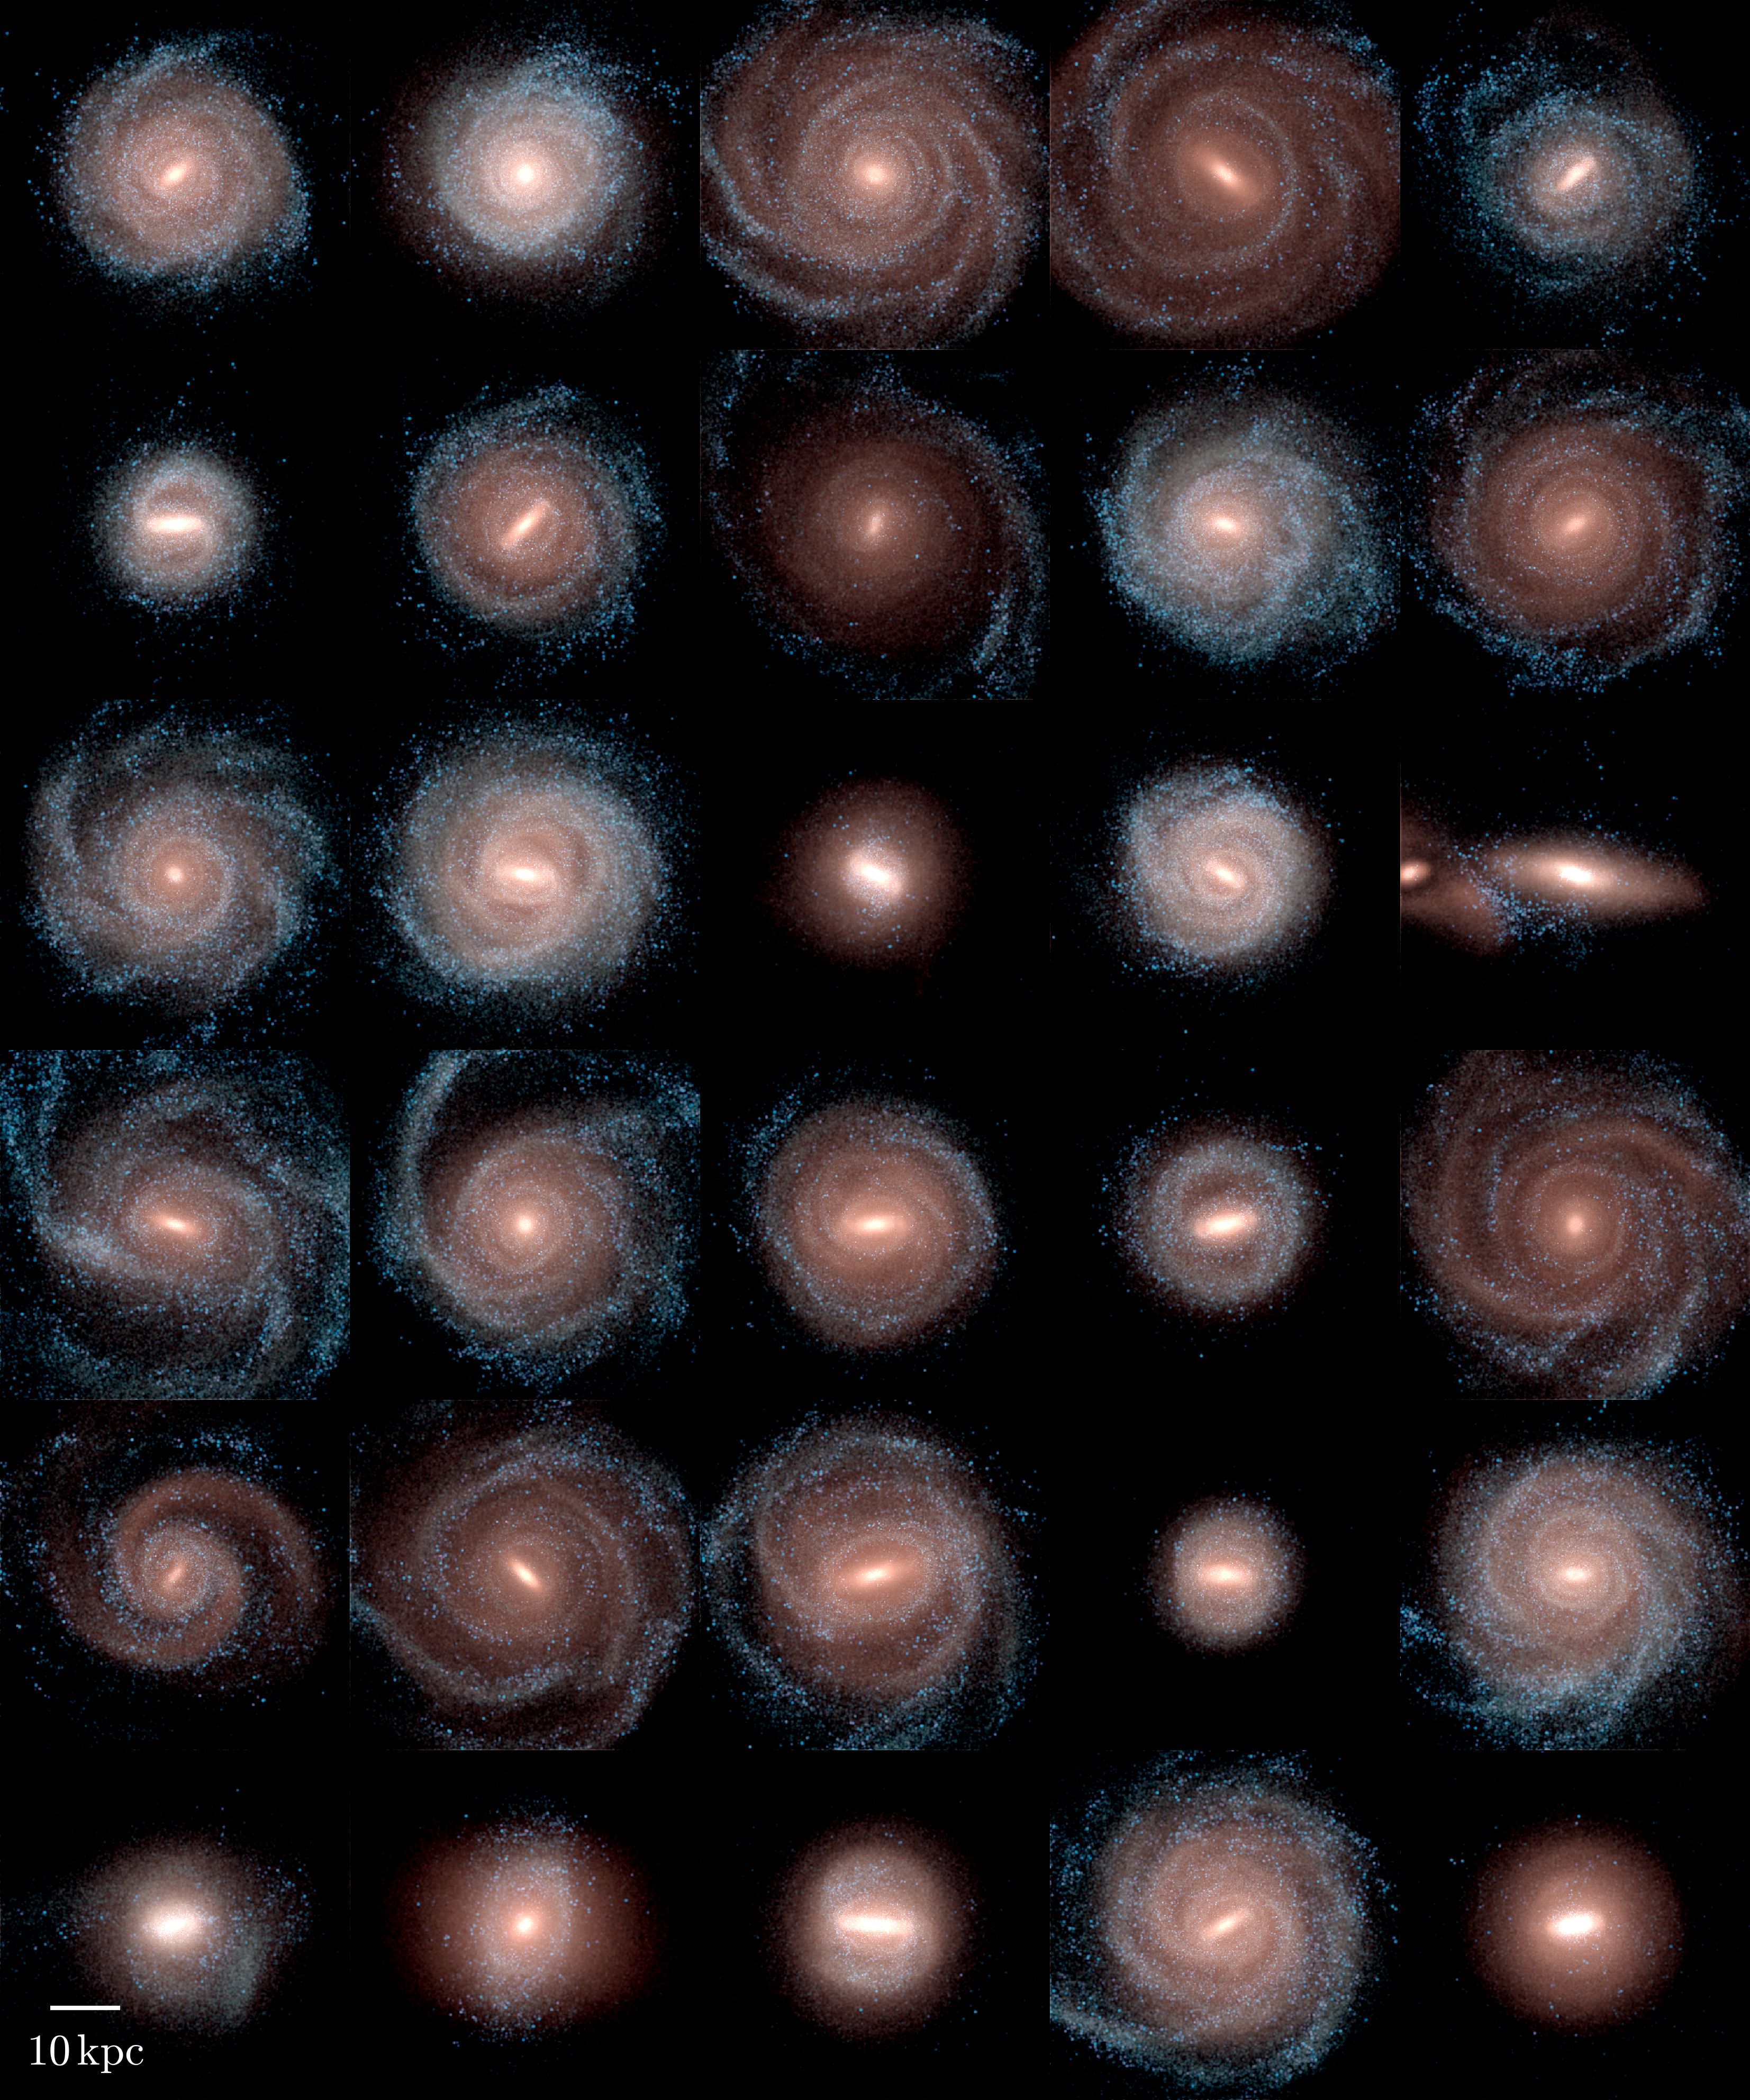
\includegraphics[width=1\linewidth]{./pics/Auriga.png}
\caption{\tiny Auriga simulations. http://auriga.h-its.org}
\end{figure}
\end{column}

\begin{column}{.6\textwidth}
\centering
\footnotesize
\begin{itemize}

\item How do they track this evolution? SPH MMH.
\item Feedback processes are one of the most important features of these simulations.
\item We focus on AURIGA \cite{auriga} simulations made with AREPO \cite{arepo}.
\item These are a set of 30 MW-like galaxies with latest physics models and hydrodynamics numerical methods.
\item Various versions of these simulations: resolution, presence of gas, presence of Magnetic Fields.
\item One of the firsts and few simulations able to implement magnetic fields

\end{itemize}

\end{column}

\end{columns}

\end{frame}

%---------------------------------------------------------------------------------------
\subsection{Example of how simulations complement observations}
\begin{frame}

A study of the shape in terms of the radius and history.

\begin{figure}[c]
\includegraphics[width=0.8\linewidth]{./pics/veraCiroAquarius.png}
\end{figure}

\end{frame}

%---------------------------------------------------------------------------------------

\begin{frame}

\begin{columns}[c]

\begin{column}{.4\textwidth}
\begin{figure}
\includegraphics[width=0.8\linewidth]{./pics/shapeRadius.png}
\caption{\tiny Dependence of shape on radius}
\end{figure}
\end{column}

\begin{column}{.7\textwidth}
\centering
\begin{figure}
\includegraphics[width=1\linewidth]{./pics/shapeHistory.png}
\caption{\tiny Dependence of shape on history}
\end{figure}

\end{column}

\end{columns}

\end{frame}

%---------------------------------------------------------------------------------------
\begin{frame}

They made this analysis on the latest set of MW-like simulations (at the time), Aquarius \cite{aquarius}.\\~\\

Shape in terms of radius? How to measure it? \\~\\

The main results are: 

\begin{itemize}
\item Dependence of the DM halo shape on the radius.

\item Correlation of history of the DM halo shape with its history.

\item DM halos are more prolate at early stages and more oblate-triaxial at late stages.

\end{itemize}

\end{frame}


%---------------------------------------------------------------------------------------
\begin{frame}

Given these results, we can now implement them on observations:

\begin{figure}[c]
\includegraphics[width=1\linewidth]{./pics/veraCiroSagitarius.png}
\end{figure}

\end{frame}

%---------------------------------------------------------------------------------------

\begin{frame}

This study is an improvement of the Law \& Majewski 2010 study in which asumptions are relaxed.\\~\\

The DM halo has the following properties:

\begin{itemize}
\item It is axisymmetric at inner parts, \textbf{coherent with the MW disk}.

\item It is triaxial on the outer-skirts following the Law \& Majewski 2010 study.

\item It has a smooth transition between those two regimes.

\end{itemize}

They used variation of parameters in simulations to obtain the best fit:

\begin{itemize}
\item DM halo is oblate with $qz = 0.9$ at $r \approx 10kpc$

\item DM halo is triaxial with $b/a = 0.9, c/a = 0.8$ at $r>>30kpc$

\end{itemize}

\end{frame}

%---------------------------------------------------------------------------------------
\section{Our study}
\subsection{Objectives}
\begin{frame}
Taking into account this introduction and the state-of-the art simulations from AURIGA, we are motivated to make an study with the following objectives.

\begin{itemize}
\item Study the shape of the DM halo in terms of the radius in the AURIGA simulations.

\item Verify that the shape of the DM halo keeps memory by studying its dependence with redshift.

\item \textbf{\textit{Analyze the relation or the effect of baryons on the DM halo shape.}}

\end{itemize}

\end{frame}

%---------------------------------------------------------------------------------------
\subsection{How we calculate DM shapes in terms of radius (simulations)}
\begin{frame}
\footnotesize
We use the method used by Vera-Ciro et al. 2011 to calculate shapes.\\~\\

Shapes are determined by the semiaxes $a,b,c$ of the ellipsoid associated to the halo.\\~\\

First we choose a radius $R$. We calculate the reduced inertia tensor for all particles within the defined sphere:

\begin{equation}
I_{ij} = \sum_k \frac{x_k^{(i)}x_k^{(j)}}{d^2_k}
\end{equation}

The eigenvalues of this tensor are said semiaxes along the corresponding eigenvectors.\\~\\
But this is not sufficient: Calculate ellipse from spherical selection of particles.

\end{frame}


%---------------------------------------------------------------------------------------
\begin{frame}
\small

The solution is to rescale positions for the current ellipse to become a sphere and recalculate:\\~\\

Once obtained the first semiaxes, we rescale:

\begin{align}
(x,y,z) &\rightarrow (x,y/q,z/s) \\
q &=  b/a\\
s &= c/a,
\end{align}

This rescaling is used to redefine the contour \textit{sphere} and to calculate the \textit{distance} in the inertia tensor.\\~\\

The semiaxes are recalculated the rescaling is performed iteratively until we achieve convergence: changes in semiaxes are less than $10^{-6}$


\end{frame}

%---------------------------------------------------------------------------------------
\subsection{Our results}

\begin{frame}[plain]

\begin{columns}[c]

\begin{column}{.5\textwidth}

\begin{figure}
\subfloat{%
  \includegraphics[clip,width=0.8\columnwidth]{./pics/halo9DM_in.png}%
}

\subfloat{%
  \includegraphics[clip,width=0.8\columnwidth]{./pics/halo9DM_out.png}%
}
\caption{\tiny DM simulation: Halo 9}

\end{figure}

\end{column}

\begin{column}{.5\textwidth}

\begin{figure}
\subfloat{%
  \includegraphics[clip,width=0.8\columnwidth]{./pics/halo9MHD_in.png}%
}

\subfloat{%
  \includegraphics[clip,width=0.8\columnwidth]{./pics/halo9MHD_out.png}%
}
\caption{\tiny MHD simulation: Halo 9}

\end{figure}


\end{column}

\end{columns}

\end{frame}

%---------------------------------------------------------------------------------------
\begin{frame}[plain]

\begin{columns}[c]

\begin{column}{.5\textwidth}
\begin{figure}
\includegraphics[width=1.1\columnwidth]{./pics/parte1.png}
\caption{\tiny Semiaxes ratios}
\end{figure}
\end{column}

\begin{column}{.5\textwidth}
\centering
\begin{figure}
\includegraphics[width=1.1\columnwidth]{./pics/parte2.png}
\caption{\tiny Semiaxes ratios and Triaxiality $\frac{a^2-b^2}{a^2-c^2}$}
\end{figure}

\end{column}

\end{columns}


\end{frame}
%---------------------------------------------------------------------------------------

\begin{frame}[plain]

\begin{columns}[c]

\begin{column}{.5\textwidth}
\begin{figure}
\includegraphics[width=1.1\columnwidth]{./pics/Triaxiality_Inner.png}
\caption{\tiny Comparison in triaxiality plane DM vs MHD at $0.01_{Rvir}$}
\end{figure}
\end{column}

\begin{column}{.5\textwidth}
\centering
\begin{figure}
\includegraphics[width=1.1\columnwidth]{./pics/Triaxiality_Outer.png}
\caption{\tiny \tiny Comparison in triaxiality plane DM vs MHD at $_{Rvir}$}
\end{figure}

\end{column}

\end{columns}


\end{frame}

%---------------------------------------------------------------------------------------

%---------------------------------------------------------------------------------------
\section{Future work}

\begin{frame}

\begin{itemize}

\item Study the historical shape\\~\\

\item Verify the effec of gas in the shape of DM halos\\~\\

\item Compare our results with previous works (observational and theoretical)\\~\\

\item Write thesis\\~\\

\end{itemize}

\end{frame}

%---------------------------------------------------------------------------------------

%---------------------------------------------------------------------------------------


%---------------------------------------------------------------------------------------

%---------------------------------------------------------------------------------------


%---------------------------------------------------------------------------------------

%---------------------------------------------------------------------------------------



\section{References}
\begin{frame}[t, allowframebreaks]
\frametitle{Referencias}
\tiny
\bibliographystyle{unsrt}
\bibliography{Bibliography}
\end{frame}
\end{document}
